\chapter{Исследовательская часть}

\section{Технические характеристики}

Технические характеристики устройства, на котором выполнялись замеры по времени представлены далее.

\begin{itemize}[label=---]
	\item Процессор: Intel(R) Core(TM) i5-10300H CPU 2.50 ГГц~\cite{intel}.
	\item Оперативная память: 16 ГБайт.
	\item Операционная система: Windows 10 Pro 64-разрядная система версией 21H2~\cite{windows}.
\end{itemize}

При замерах времени ноутбук был включен в сеть электропитания и был нагружен только системными приложениями.

\clearpage

\section{Демонстрация работы программы}

На рисунке \ref{img:demonstration} представлена демонстрация работы разработанного приложения для алгоритмов сортировок, у которого имеется консольное меню для выбора запуска одного или всех алгоритмов или процесс замера по времени работы алгоритмов. На данном примере представляется, что при выборе алгоритма пользователю позволяется выбрать самостоятельный ввод данных или генерацию случайных данных по указанному размеру матрицы после чего выполняется выбранный алгоритм. 

\begin{figure}[h]
	\centering
	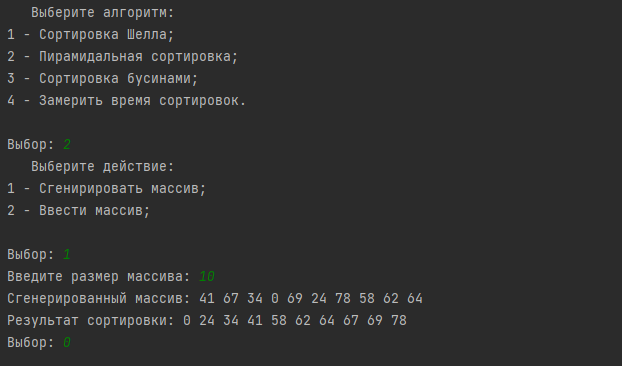
\includegraphics[height=0.35\textheight]{img/example.png}
	\caption{Демонстрация работы программы}
	\label{img:demonstration}
\end{figure}

\section{Временные характеристики}

Результаты эксперимента замеров по времени приведены в \newline таблицах \ref{tbl:time_sort} -- \ref{tbl:time_rsort}.

В таблице \ref{tbl:time_sort} приведены результаты замеров по времени лучшего случая для сортировки Шелла и пирамидальной сортировки, то есть это отсортированный массив данных по возрастанию. Лучшим случаем для сортировки Бусинами является массив с элементами минимального значения, размером от 50 до 1000 с различным шагом, то есть [50; 100] с шагом 50 и [100; 1000] с шагом 100.

\begin{table}[ht]
	\small
	\begin{center}
		\begin{threeparttable}
		\caption{Замеры по времени лучшего случая для сортировок, размер которых от 50 до 1000.}
		\label{tbl:time_sort}
		\begin{tabular}{|c|c|c|c|}
			\hline
			& \multicolumn{3}{c|}{\bfseries Время, мс} \\ \cline{2-4}
			\bfseries Количество элементов & \bfseries Шелла & \bfseries Пирамидальный & \bfseries Бусинами
			\csvreader{csv/sort_time.csv}{}
			{\\\hline \csvcoli & \csvcolii & \csvcoliii & \csvcoliv} \\
			\hline
		\end{tabular}
		\end{threeparttable}
	\end{center}
\end{table}

По таблице \ref{tbl:time_sort} был построен графики \ref{plt:sort_1} и \ref{plt:sort_2}, в котором показан лучший обзор сравнения сортировки Шелла и пирамидальной сортировки. Исходя из этих данных можно понять, что лучшего всего в этом случае работает сортировка Шелла. При этом разница во времени между пирамидальной сортировкой и сортировкой Шелла в 2 раза, а хуже всего работает сортировка бусинами в 100-200 раз, чем остальные сортировки.

\clearpage

\begin{figure}[h]
	\centering
	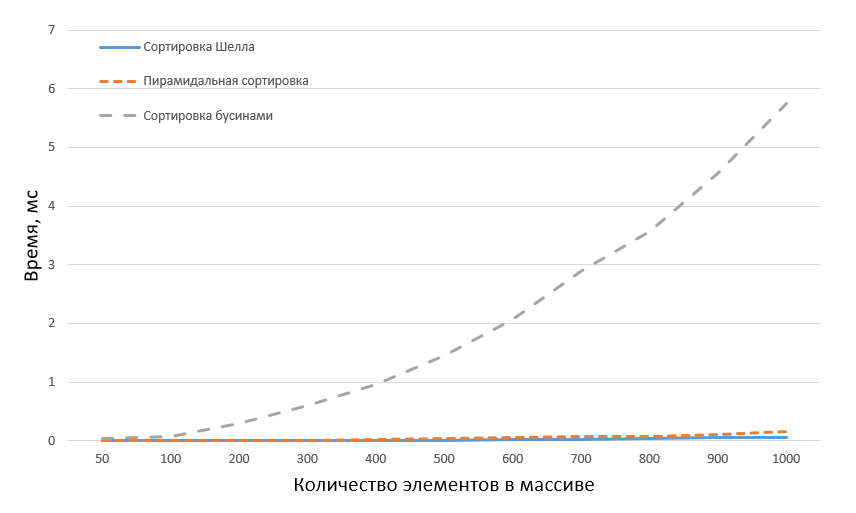
\includegraphics[height=0.3\textheight]{img/sort_1.png}
	\caption{Сравнение по времени сортировок Шелла, пирамидальную и бусинами с входным отсортированным массиве по возрастанию}
	\label{plt:sort_1}
\end{figure}

\begin{figure}[h]
	\centering
	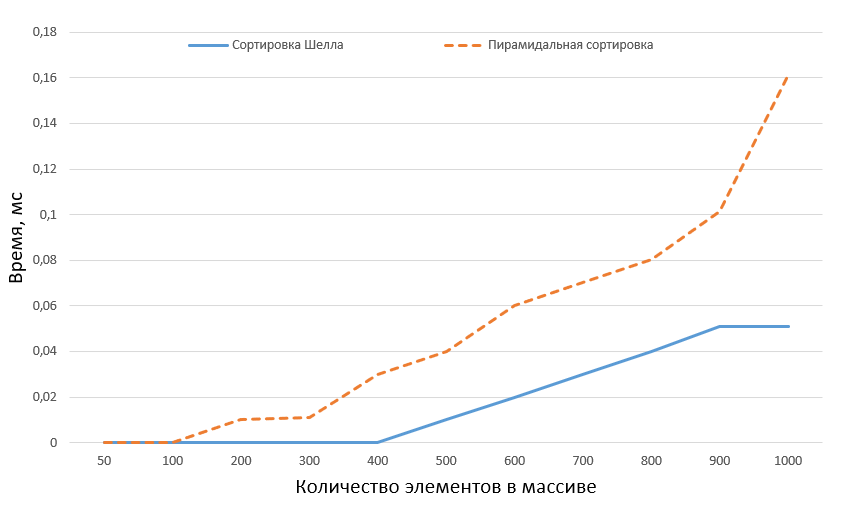
\includegraphics[height=0.3\textheight]{img/sort_2.png}
	\caption{Сравнение по времени сортировок Шелла и пирамидальную с входным отсортированным массиве по возрастанию}
	\label{plt:sort_2}
\end{figure}

В таблице \ref{tbl:time_random} приведены результаты замеров по времени для сортировки Шелла, пирамидальной сортировки и сортировки бусинами, где на вход поступает отсортированный по возрастанию массив данных размером от 50 до 1000 с различным шагом, то есть [50; 100] с шагом 50 и [100; 1000] с шагом 100.

\clearpage

\begin{table}[ht]
	\small
	\begin{center}
		\begin{threeparttable}
		\caption{Замеры по времени, размер которых от 50 до 1000, с входным случайным массивом}
		\label{tbl:time_random}
		\begin{tabular}{|c|c|c|c|}
			\hline
			& \multicolumn{3}{c|}{\bfseries Время, мс} \\ \cline{2-4}
			\bfseries Количество элементов & \bfseries Шелла & \bfseries Пирамидальный & \bfseries Бусинами
			\csvreader{csv/sort_time.csv}{}
			{\\\hline \csvcoli & \csvcolii & \csvcoliii & \csvcoliv} \\
			\hline
		\end{tabular}
		\end{threeparttable}
	\end{center}
\end{table}

По таблице \ref{tbl:time_random} был построен график \ref{plt:random}. Исходя из этих данных можно понять, что лучшего всего в этом случае работает сортировка Шелла. При этом разница во времени между пирамидальной сортировкой и сортировкой Шелла незначительна в 1,5 раза, а хуже всего работает сортировка бусинами в 50-100 раз, чем остальные сортировки.

\begin{figure}[h]
	\centering
	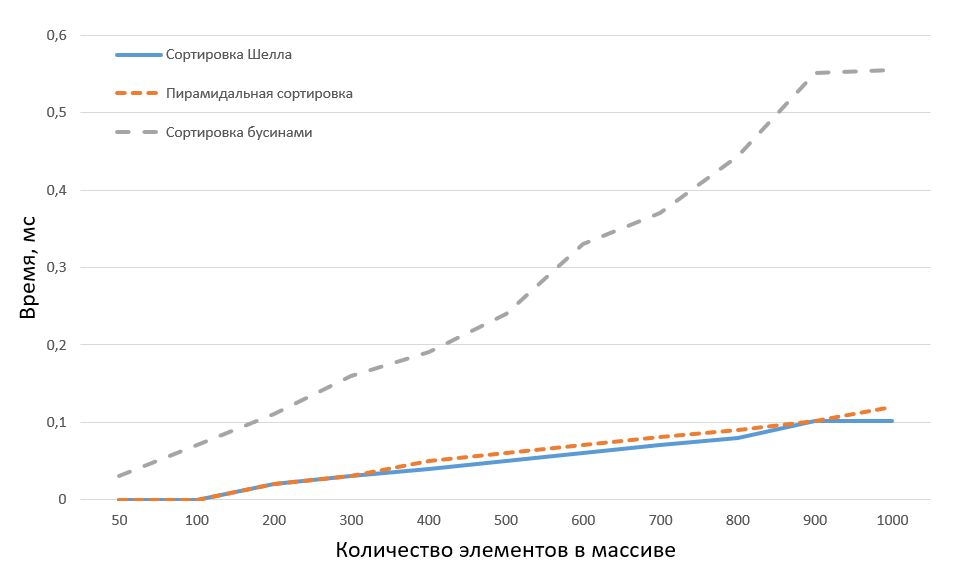
\includegraphics[height=0.3\textheight]{img/random.png}
	\caption{Сравнение по времени сортировки Шелла, пирамидальной и бусинами с входным случайным массивом}
	\label{plt:random}
\end{figure}

В таблице \ref{tbl:time_rsort} приведены результаты замеров худшего случая по времени для сортировки Шелла, пирамидальной сортировки и сортировки бусинами, то есть для сортировок Шелла и пирамидальной это случаи, когда массив отсортирован по убыванию (в обратном порядке сортировки), а для сортировки бусинами учтены большие данные, так как на вход поступает массив целых чисел, то это числа больше 1000. При замерах по времени  размер входного массива поступал от 50 до 1000 с различным шагом, то есть [50; 100] с шагом 50 и [100; 1000] с шагом 100.

\begin{table}[ht]
	\small
	\begin{center}
		\begin{threeparttable}
		\caption{Замеры по времени, размер которых от 50 до 1000, с входным отсортированным массивом по убыванию}
		\label{tbl:time_rsort}
		\begin{tabular}{|c|c|c|c|}
			\hline
			& \multicolumn{3}{c|}{\bfseries Время, мс} \\ \cline{2-4}
			\bfseries Количество элементов & \bfseries Шелла & \bfseries Пирамидальный & \bfseries Бусинами
			\csvreader{csv/rsort_time.csv}{}
			{\\\hline \csvcoli & \csvcolii & \csvcoliii & \csvcoliv} \\
			\hline
		\end{tabular}	
		\end{threeparttable}
	\end{center}
\end{table}

По таблице \ref{tbl:time_random} был построен графики \ref{plt:rsort_1} и \ref{plt:rsort_2}, в котором показан лучший обзор сравнения сортировки Шелла и пирамидальной сортировки. Исходя из этих данных можно понять, что лучшего всего в этом случае работает пирамидальная сортировка. При этом разница во времени между пирамидальной сортировкой и сортировкой Шелла незначительна в 1,5 раза, а хуже всего работает сортировка бусинами в 500 раз, чем остальные сортировки.

\clearpage

\begin{figure}[h]
	\centering
	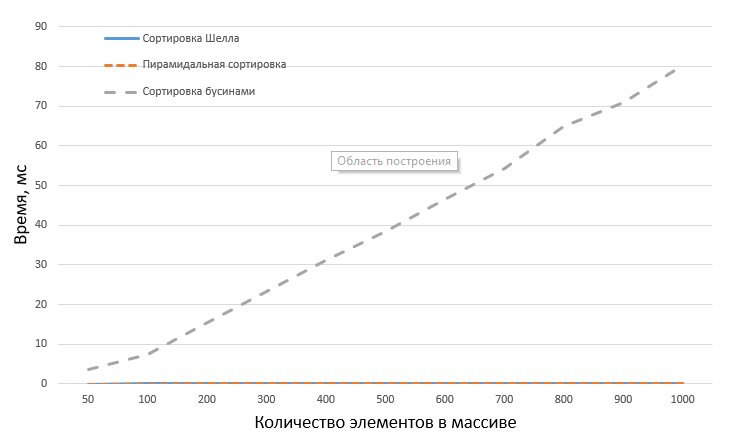
\includegraphics[height=0.3\textheight]{img/rsort_1.png}
	\caption{Сравнение по времени сортировок Шелла, пирамидальной и бусинами с входным отсортированным массивом по убыванию}
	\label{plt:rsort_1}
\end{figure}

\begin{figure}[h]
	\centering
	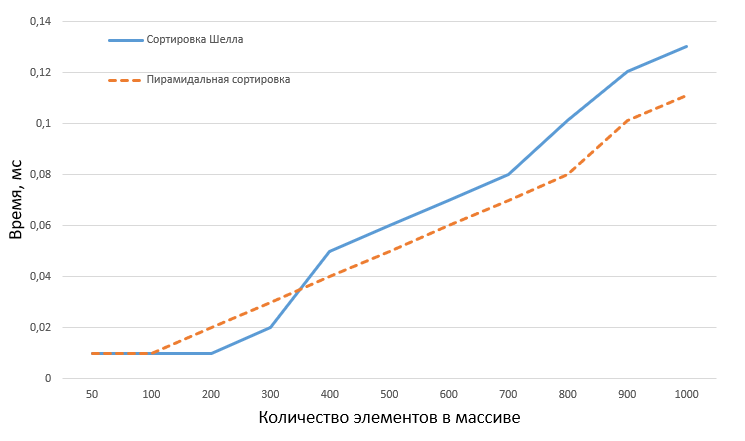
\includegraphics[height=0.3\textheight]{img/rsort_2.png}
	\caption{Сравнение по времени сортировок Шелла и пирамидальной с входным отсортированным массивом по убыванию}
	\label{plt:rsort_2}
\end{figure}

\clearpage

\section{Вывод}
В данном разделе было произведено сравнение количества затраченного времени вышеизложенных алгоритмов. Наименее затратным по времени оказался сортировка Шелла для отсортированного массива по возрастанию и пирамидальная сортировка для отсортированного массива по убыванию, а худшей сортировкой оказалась сортировка бусинами в сравнении с остальными сортировками.

Приведенные временные характеристики показывают, что лучшей сортировкой при работе с отсортированным массивом по возрастанию является сортировка Шелла, а при работе с отсортированном массиве по убыванию (в обратном порядке для сортировки) является пирамидальная сортировка. Сортировка бусинами же показала худшие результаты по сравнению с сортировкой Шелла и пирамидальной в 50-500 раз взависимости от входных данных.
